\section{Results and Proposed Approach}

\subsection{Overview}

\begin{figure}[t]
    \centering
    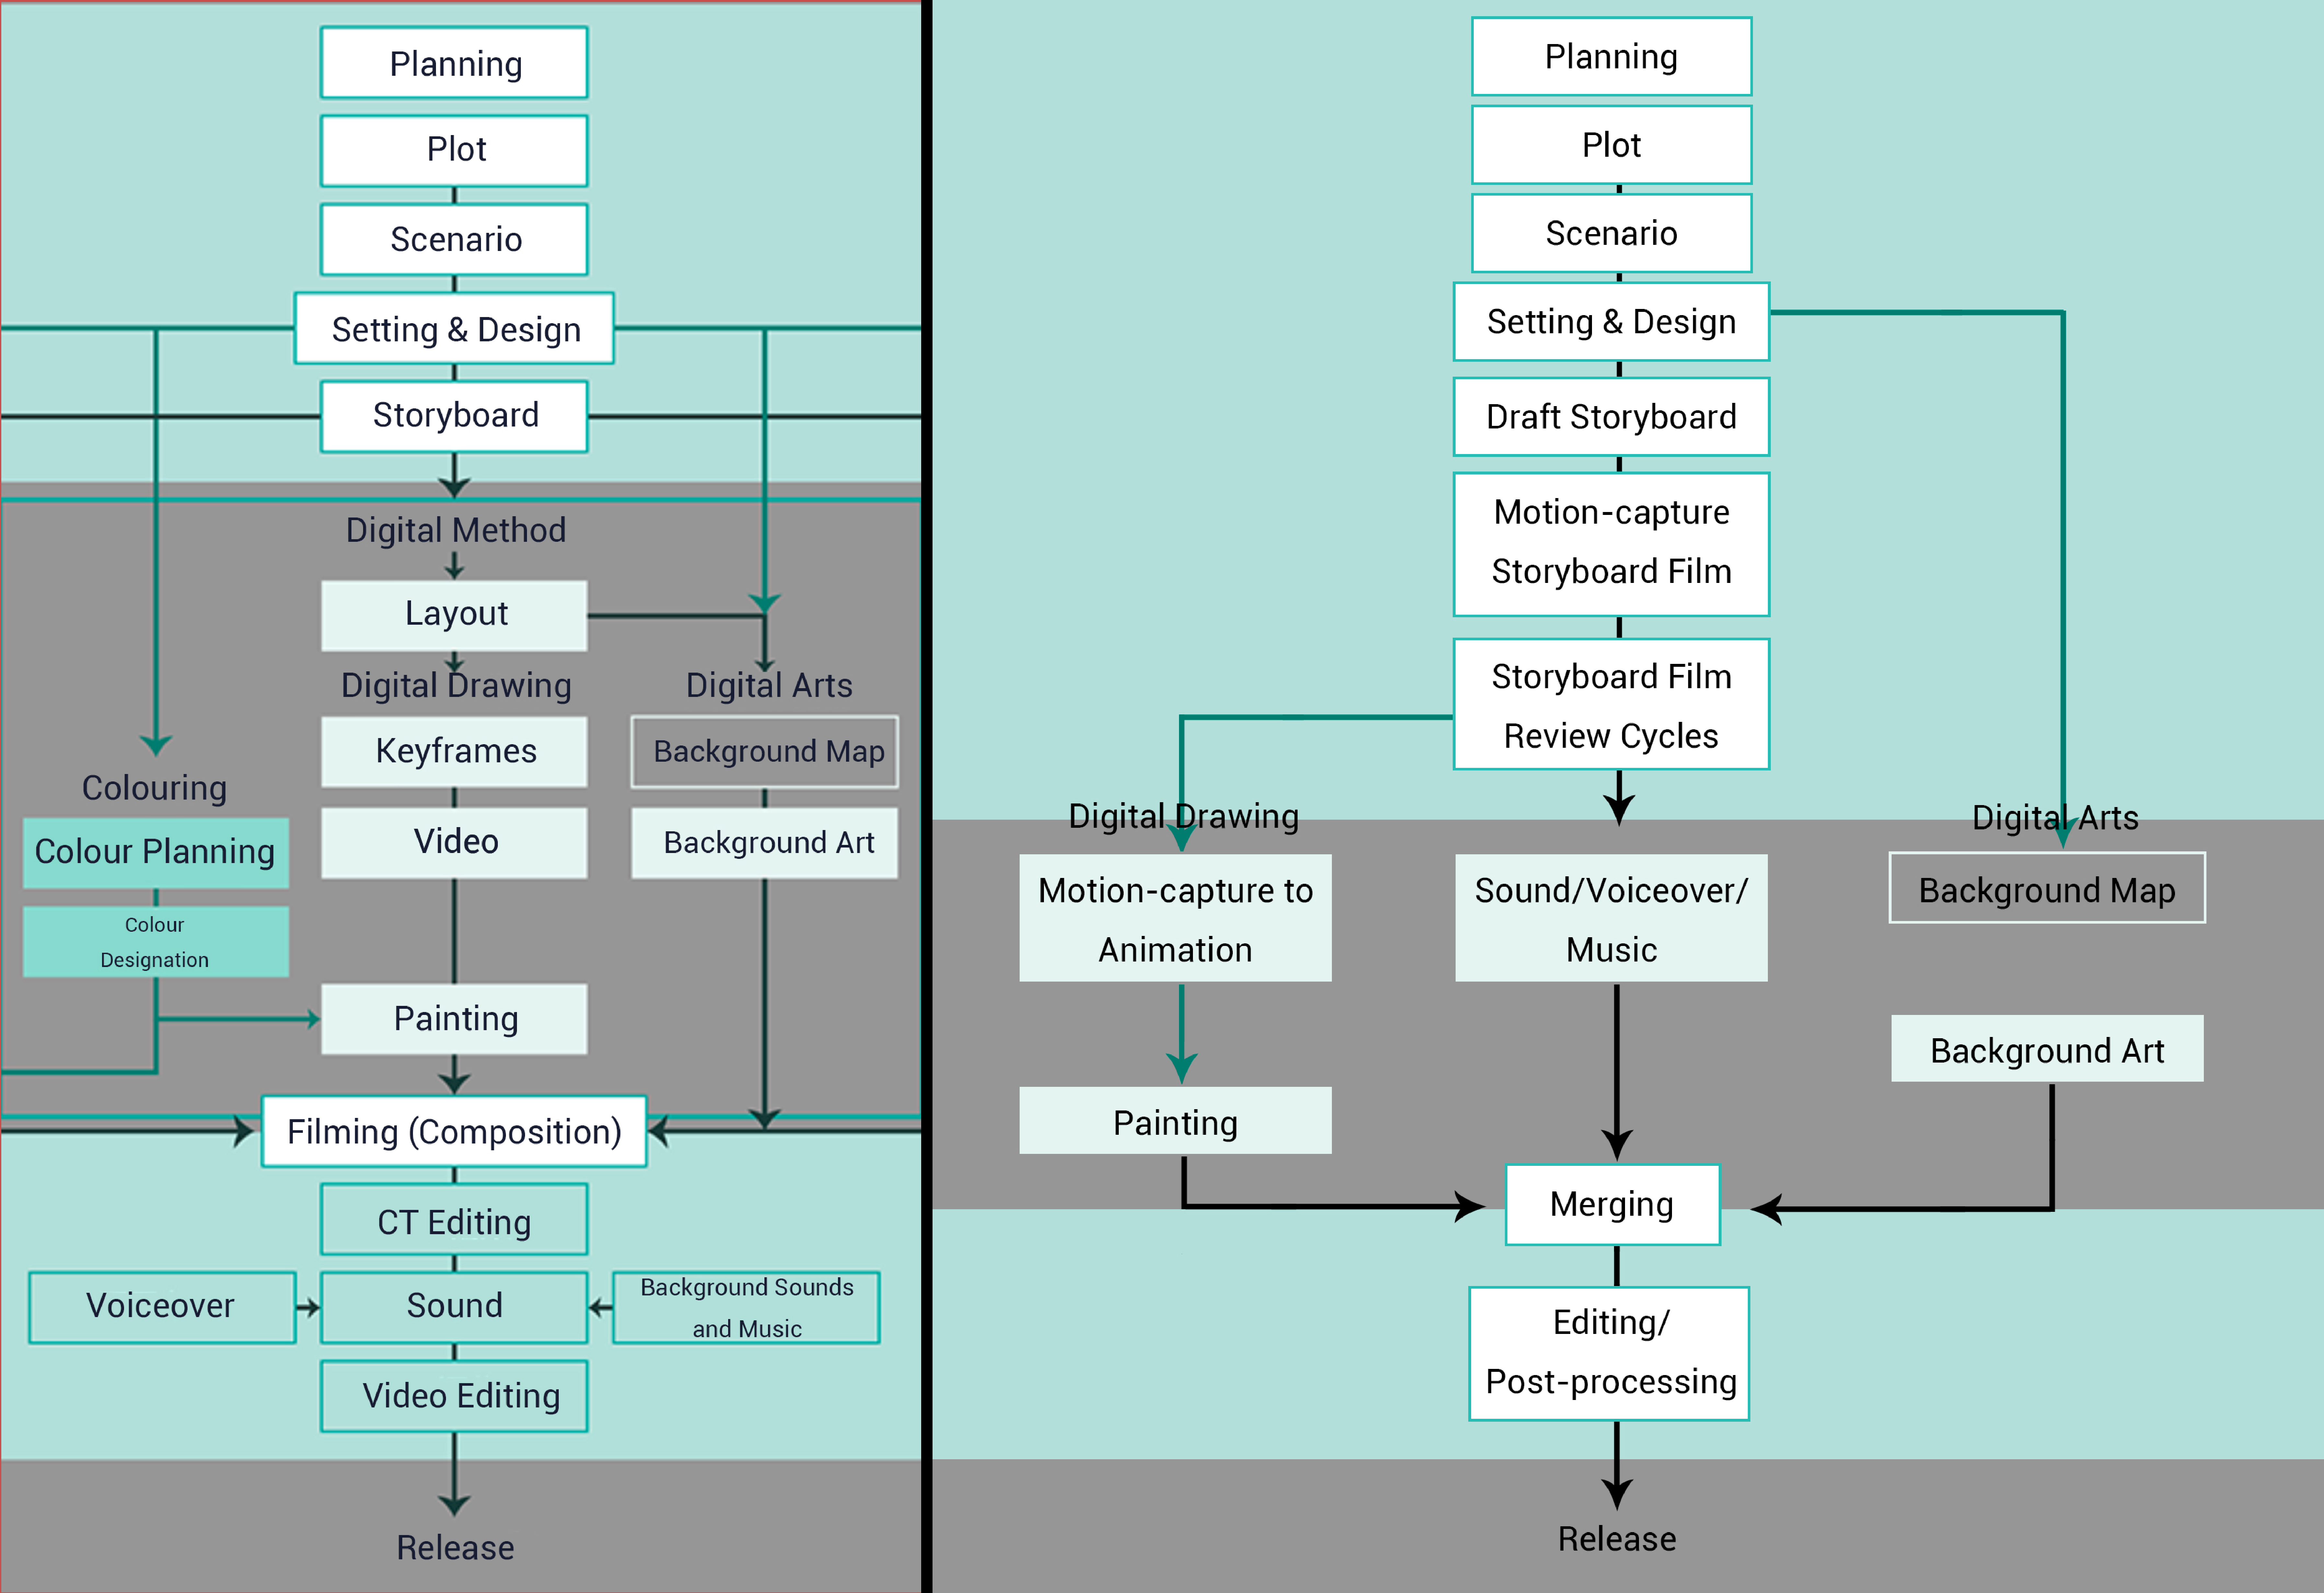
\includegraphics[width=1\linewidth]{img/results/workflow.pdf} \\
    \caption{\textbf{Left:} Current industry anime production process~\cite{animeProcessAutodesk}. \textbf{Right:} Reworked process used with Brighter the Animation.}
    \vspace{-15pt}
    \label{fig:workflow}
\end{figure}

The current anime production process can be divided into the following steps~\cite{animeProcess, animeProcessAutodesk}:

\begin{enumerate}
    \item Pre-production
        \begin{enumerate}[label*=\arabic*.]
            \item Planning
            \item Plot
            \item Scenario
            \item Setting \& Design
            \item \textbf{Output for next stage:} Storyboard
        \end{enumerate}
    \item Production (done in parallel)
        \begin{enumerate}[label*=\arabic*.]
            \item Colour Planning
            \item Drawing (Line Animation)
            \item Backgrounds
            \item \textbf{Output for next stage:} Painting to Composition
        \end{enumerate}
    \item Post-processing
        \begin{enumerate}[label*=\arabic*.]
            \item CT Editing (cuts)
            \item Sounds (voiceover, background, music)
            \item Video Editing
            \item \textbf{Output for next stage:} Release
        \end{enumerate}
\end{enumerate}

In this case, each stage is a pre-requisite of the next one, meaning Dubbing cannot start until all the items in Production are completed. Taking these and the references into account, a new pipeline is used for creating Brighter the Animation:

\begin{enumerate}
    \item Pre-production
    \begin{enumerate}[label*=\arabic*.]
        \item Planning
        \item Plot
        \item Scenario
        \item Setting \& Design
        \item Draft Storyboard
        \item Motion-capture Storyboard Film
        \item Storyboard Film Review Cycles
        \item \textbf{Output for next stage:} Storyboard Film
    \end{enumerate}
    \item Production (done in parallel)
    \begin{enumerate}[label*=\arabic*.]
        \item Drawing (Line Animation) to Painting
        \item Sound/Voiceover/Music
        \item Backgrounds
        \item \textbf{Output for next stage:} Merged Animation Draft
    \end{enumerate}
    \item Post-processing
    \begin{enumerate}[label*=\arabic*.]
        \item Video Editing/Post Processing
        \item \textbf{Output for next stage:} Release
    \end{enumerate}
\end{enumerate}

\begin{figure}[t]
    \centering
    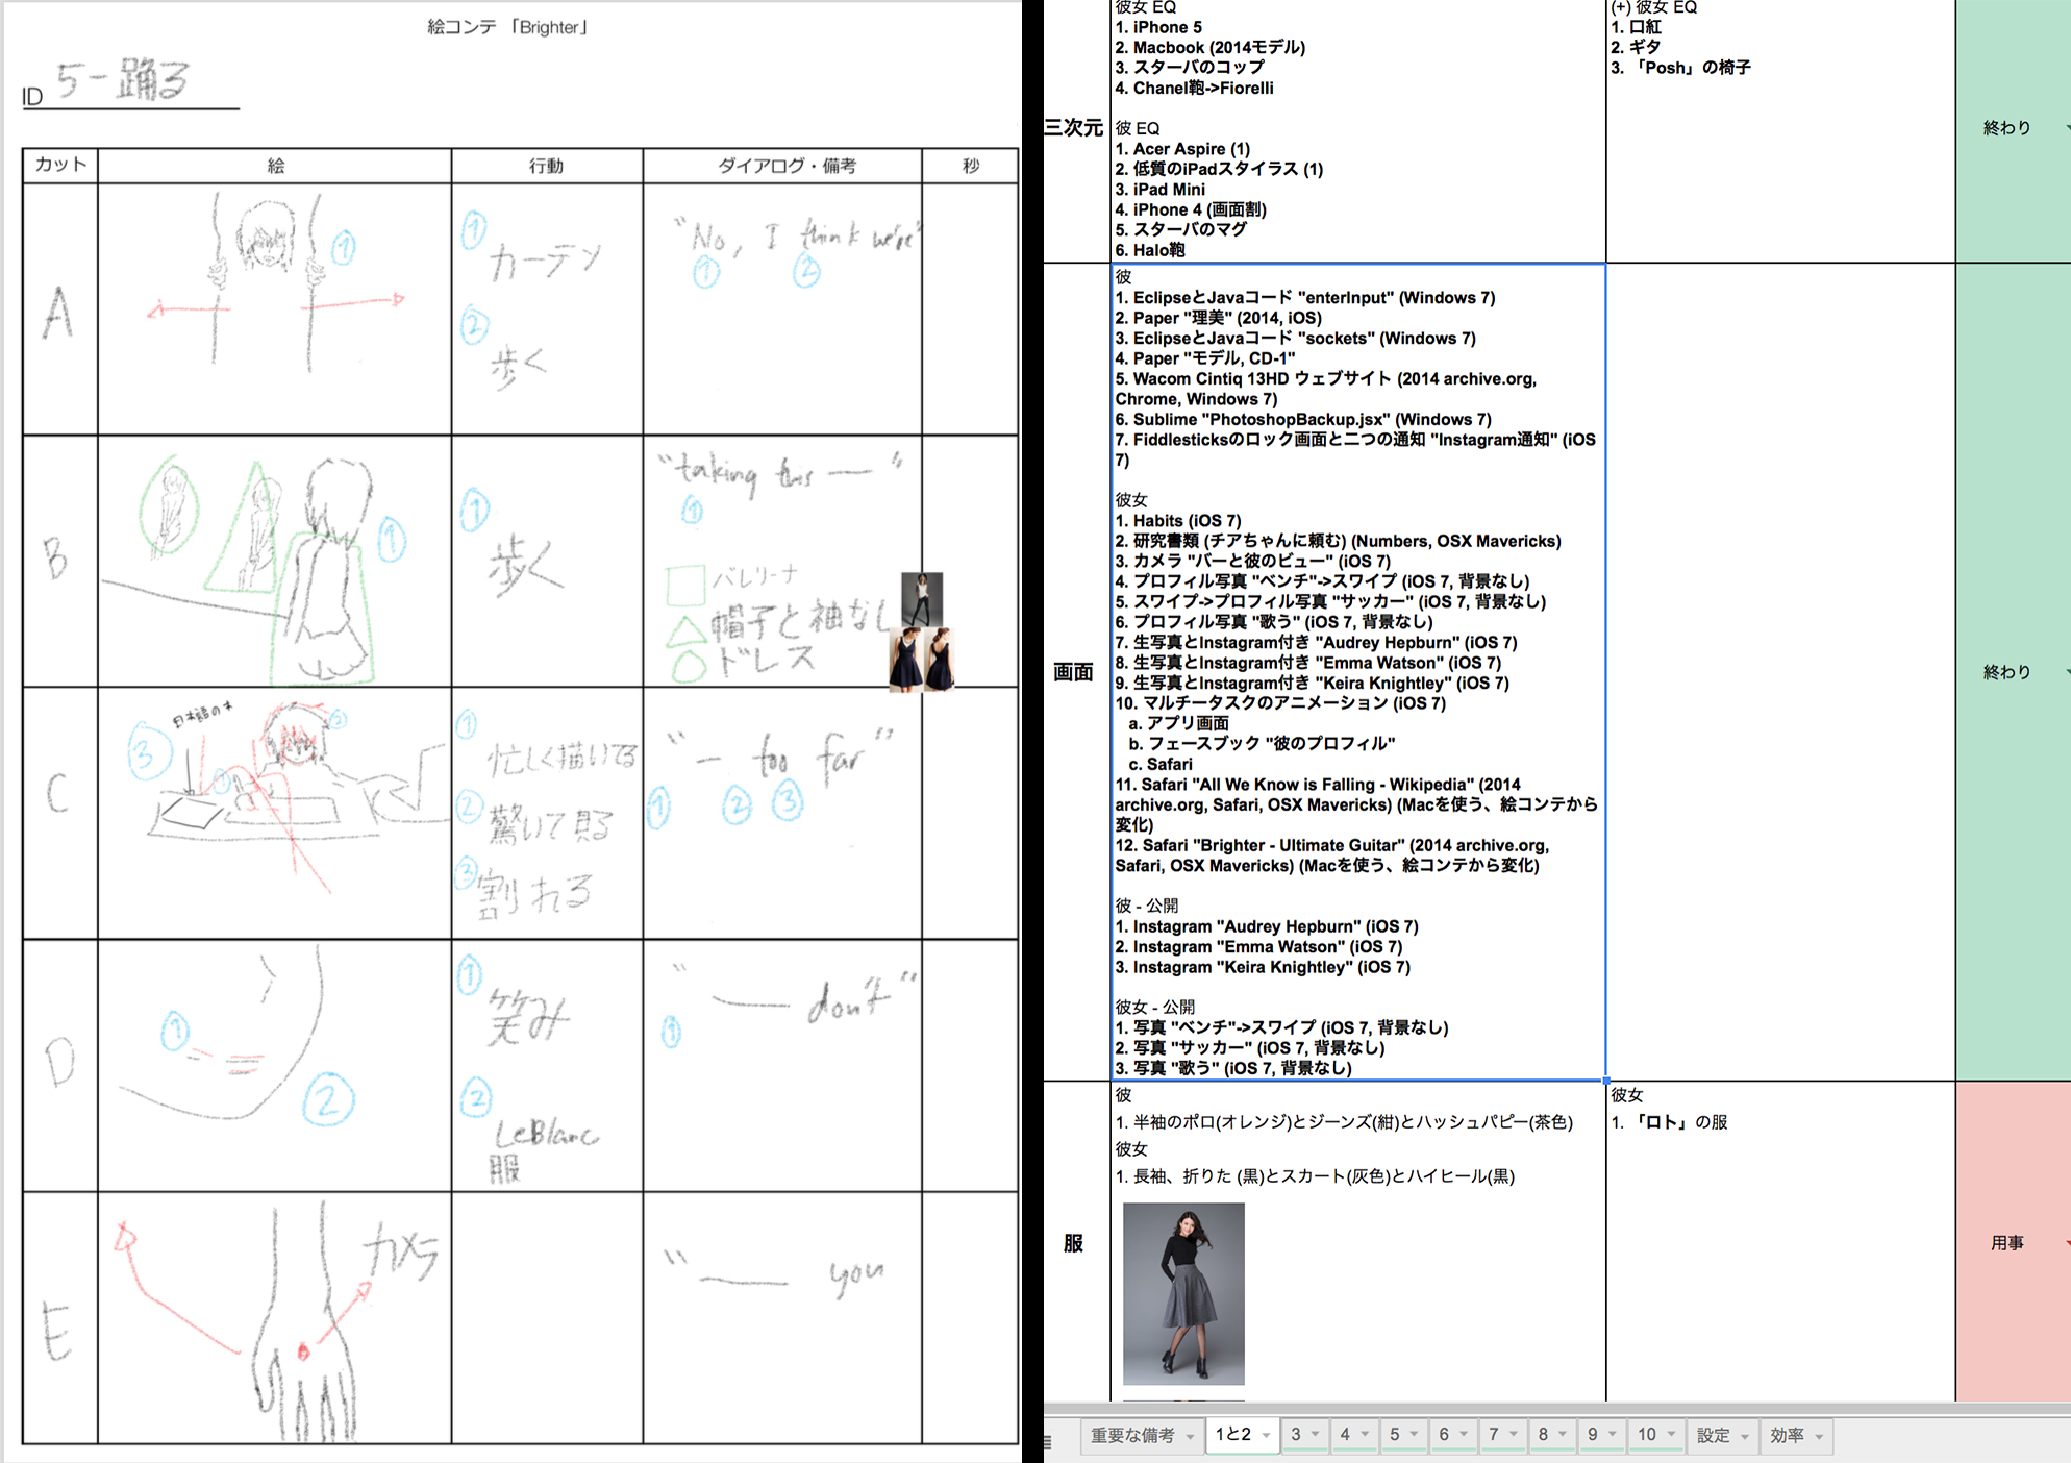
\includegraphics[width=1\linewidth]{img/results/storyboard.pdf} \\
    \caption{\textbf{Left:} Draft, quick-drawn storyboard page. \textbf{Right:} Spreadsheet for object and costume list organised for each scene.}
    \vspace{-15pt}
    \label{fig:storyboard}
\end{figure}

This new pipeline adds steps on the pre-production stage, but by introducing this, the ability to concurrently do the visual and non-visual steps can be done, and due to the review stage in Pre-production, all stakeholders can provide inputs to improve the quality of the finalised storyboard. This prevents any unnecessary back-and-forth changes in the Production stage where the storyboards need to be rework after drawing the actual keyframes, or even the painted animations. In addition, key-frame and key-in animations for the characters can be more easily integrated since the 3D models with human-based movements can now be used as direct basis, as well as doing the CT Editing (cuts) as early as this stage. Lastly, since motion-capture is introduced in Pre-production rather than rotoscoping, a single actor, which can also be the same person as the director, can act out all the characters. In addition, if the director is the same person as the actor, similar to how Brighter the Animation was created, it is much easier for the director to record and portray how the final output and vision should be implemented. This requires additional skill on the director/actor's part, but saves more time (and ultimately expenses in a commercial environment).\\\\
Kindly note, that Brigher the Animation is a music video and is constrained to the actual music, meaning that each the drum beats and music are treated as the dubbing and sounds that have been added before completing the storyboard. This also contributed positively to having more detailed scenes that go in sync with each drum beat after meticulous storyboarding. However, Further research and application of the pipeline into an full animation that incorporates sounds, ambient music and dubbing is needed. This will be introduced in Phase 2 of the research.

\subsection{Pre-production Stage}

\begin{figure}[t]
    \centering
    \includegraphics[width=1\linewidth]{img/results/char.pdf} \\
    \caption{\textbf{Top:} Hand-drawn character designs for the unnamed heroine and male side-character. \textbf{Bottom:} Rigged skeleton models in Blender3D.}
    \vspace{-15pt}
    \label{fig:workflow}
\end{figure}

The writing, setting, character designs, and draft (paper) storyboard have been created from scratch.

Due to financial limitations, use of actual production-level motion capture devices have not been tested. In line with this, a number of experiments with different motion capture/semi-rotoscoping methods for Brighter the Animation have been used:

\begin{enumerate}
    \item Kinect V2 to NI-Mate~\cite{niMate} to Blender Rigify (NG)\\
    This method is perfect for large actions such as dance and walking for minimal characters. However, hand movements are not accurate enough to be used as actual reference. Despite the fluidity of all other parts of the rig, the hands need to be drawn from scratch for each frame. This counted as a failure case and was not used in the short film.

    \item Superimposing (Used, but not recommended)\\
        Due to the failure of Method 1, the initial part of the short film used actual video frames that have been re-sized to roughly fit the characters' proportions. These frames have been used for the body, and the head is based on the rough 3D models moved using Rigify on Blender to follow the video.\\
        This, however, made the proportions of the characters look inconsistent as shown in the images.

    \begin{figure}[t]
        \centering
        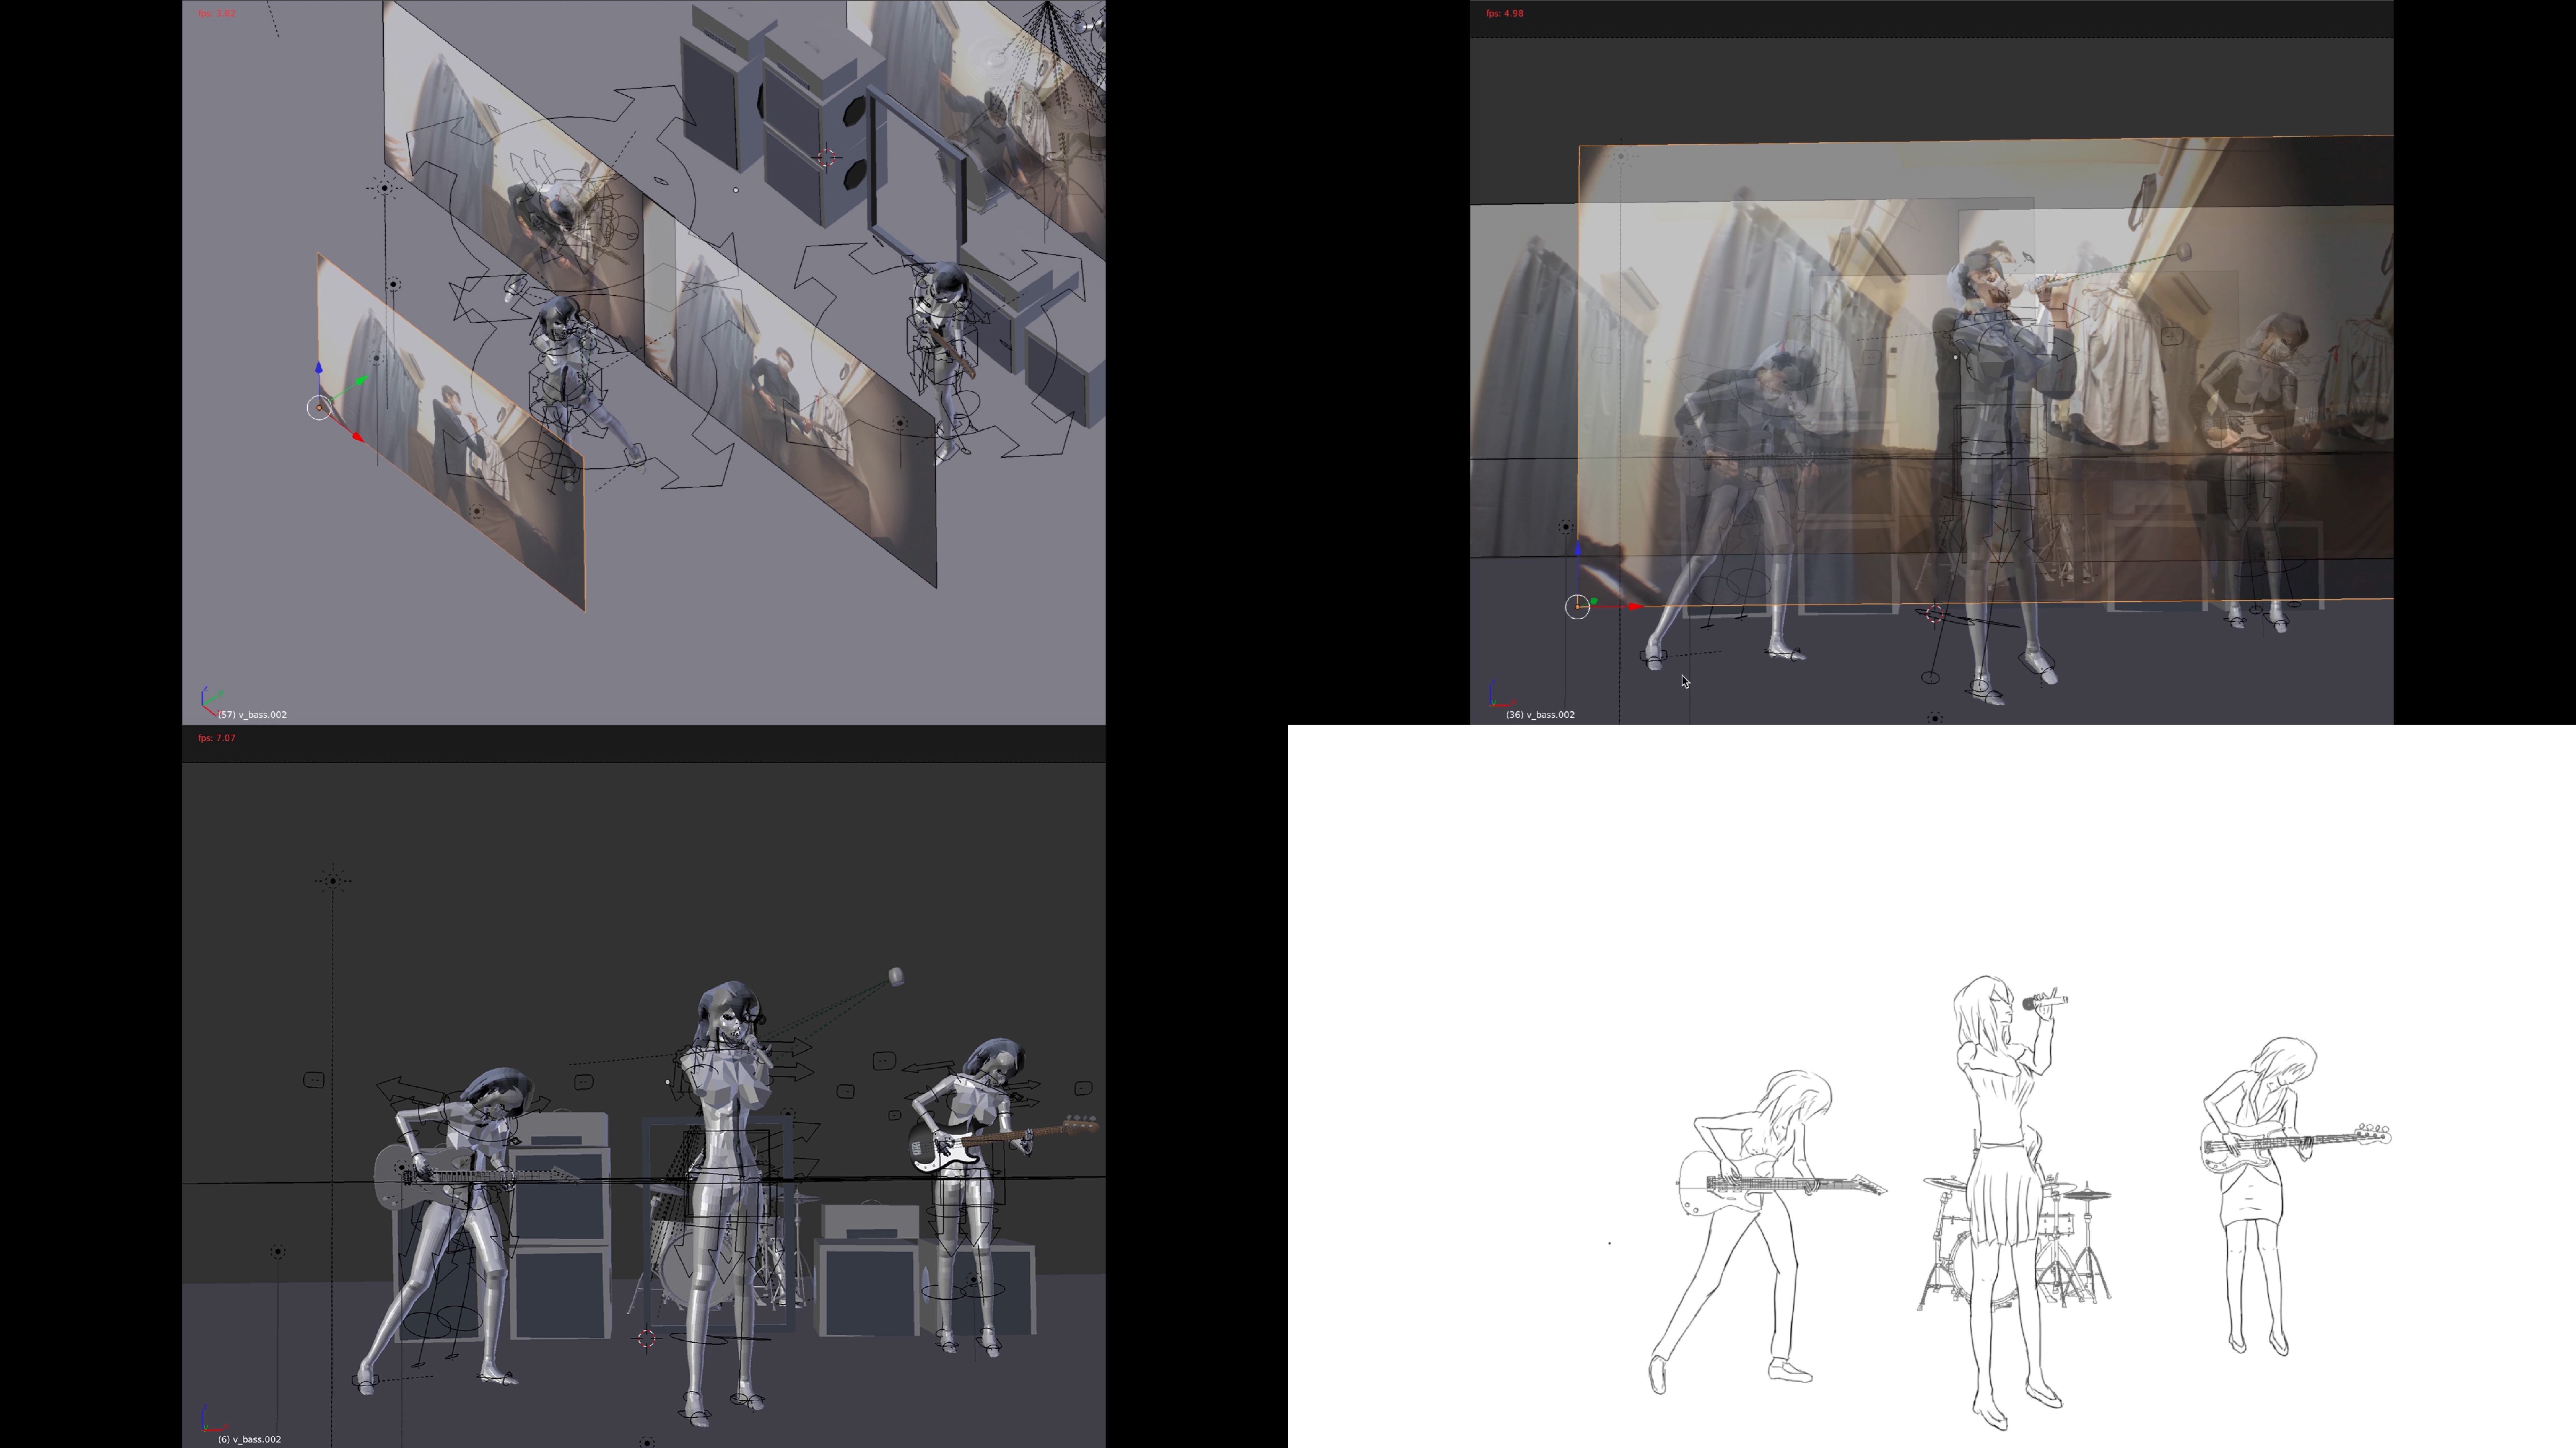
\includegraphics[width=1\linewidth]{img/results/process.pdf} \\
        \caption{\textbf{Top-left:} Angled view of 3D skeleton movement based on video. \textbf{Top-right:} Front view of 3D skeleton movement based on video. {Bottom-left:} 3D skeletons with interacted objects. {Bottom-right:} Drawn-over 3D skeletons with Freestyle-rendered objects.}
        \vspace{-15pt}
        \label{fig:process}
    \end{figure}

    \item Video reference to Rigify in Blender (Used, but actual motion capture device is more efficient)\\
        After the failure of Method 2, a new method has been created based on how motion capture automates video to 3D model movements. Due to the lack of hardware, this step was manually done by using the videos as a reference~\cite{videoToRigRef}. This, however, serves as a good benchmark for the potential of the use of motion capture hardware with finalising storyboards and keyframes. This method has been used for the remainder of the short film.

    \item Deep learning libraries for motion capture (OpenPose)~\cite{openposeArxiv}(NG)\\
    There is a famous library called OpenPose that makes use of neural networks to estimate poses directly from video. This showed great potential, but after further study and trials, the following issues proved that this is not currently a viable solution:
        \begin{itemize}
            \item The output keypoints (.json) of the library is only 2D and cannot be used in 3D software as without heavy remapping with calculus-based methods
            \item There is a 3D keypoint that requires multiple cameras, but this requires the purchase of multiple FLIR cameras~\cite{flirCamera} setup to record motion
            \item Despite the library being open-source, commercial use of the library requires \$25,000 per year~\cite{openPoseCommercial}\\
            Due to these issues, simply buying a mid-level Perceptron Neuron motion capture device for \$1500~\cite{perceptionNeuron} shows much more potential for this paper's use case than using a commercial version of the library.
        \end{itemize}
\end{enumerate}

Based on the steps above, a finalised storyboard with all the transitions and keyframes based on the 3D models moved with motion capture can be created even before the actual drawing, and can be reviewed easily for any major changes before passing it on to the Production stage. In addition, the advantage of motion capture to simple rotoscoping is the ability for the camera view to be dynamically changed in the 3D software, giving much more freedom on how the scenes can be shown.\\\\
The limitation for this is that mocap is limited to characters. Objects are still created manually. However, these can be modularised using cel shading of 3d objects to make them backgrounds~\cite{mclelunBg} and objects~\cite{mclelun3d} look more like painted anime background. More on this topic in the Production stage.

\subsection{Production Stage}

After the completion of the finalised storyboards, this stage is simply referencing the 3D movements as actual keyframes and keyin frames for animation. Drawing and animation ability is still essential in this stage, as details with both the movement and character such as clothing, hair, and physics is still taken into account. This, however, solves the following issues:
\begin{enumerate}
    \item Proportion and consistency
        \begin{itemize}
            \item Proportion and consistency in drawings is difficult to master for one person, and having a consistent proportion for characters if drawn by multiple animators is a minute detail issue with anime~\cite{dragonballInconsistency}
            \item Incorporating the CS concept of functions where having reusability for repetitive actions exponentially decreases feedback loop with both drawing and animation
        \end{itemize}
    \item Learning
        \begin{itemize}
            \item Training and onboarding for new animators is much easier as practicing the characters' proportions is already eliminated
        \end{itemize}
    \item Efficiency and work environment
        \begin{itemize}
            \item Having automation for lower level, repetitive process provides more time for a work-life balance for animators, which allows them to actually live life outside of work and incorporate those experiences into improving their craft
            \item Since training and work hours can be improved with these methods, it is now possible to actually hire less people that are full-time instead of paying lower-than-minimum wage~\cite{animatorPayLessThanMcdonalds}
            \item With more time, additional details for the art can be introduced
            \item This also includes handling of emergency cases; in the animation industry, it is very difficult to take vacation leaves because someone always needs to be able to fill in\cite{starDisneyAnimator}
        \end{itemize}
\end{enumerate}

In addition to these, further research can be done for training machine learning models, particularly Generative Adversarial Networks to quickly convert the rendered 3D models into actual anime-style in the future once enough data is created. Inputs can include the rig position, camera view, and actual frame pixels that can be run on a series of convolutional and recurrent neural networks for the generator, and have these outputs run on a discriminator. This is merely a hypothesis but the potential of this is worth noting.\\\\
As discussed in the previous section, the backgrounds and objects can be recreated with cel shading and painting-style filters. In animation, especially in films, adding a good number of visual cues is essential for portraying a story, so simply using a photo as a background is nore entirely viable. This is precisely why Makoto Shinkai's semi-rotoscoped backgrounds are not simply traceovers of the videos, but are actually modified versions of the reference frames that include more detail and reworked objects.\\\\

\begin{figure}[t]
    \centering
    \includegraphics[width=1\linewidth]{img/results/shinkai.pdf} \\
    \caption{\textbf{Top-left:} {{Real-life photo of myself at Yotsuya Station in Tokyo (taken by Jayzon Ty)}}. \textbf{Bottom-right:} Same view in Shinkai Makoto's film Kimi no Na Wa (2016). \textbf{Top-right:} {{Real-life photo of a temple near Nijo Station in Kyoto (taken by myself)} \textbf{Lower-left:} {{Same photo as top-right ran through a pre-trained Generative Adversarial Network by Chen et. al~\cite{cartoonGAN}}}.}}
    \vspace{-15pt}
    \label{fig:shinkai}
\end{figure}

This, however, is mostly for feature films that focus more on art. For more industry-level anime such as advertisements where it is more important to focus on the product rather than minute details, there are some techniques that can be used to speed up the process with the use of actual photos. An example of this is the use of trained Generative Adversarial Networks for converting photos into actual Makoto Shinkai-, Hayao Miyazaki-, and Mamoru Hosoda-style-looking backgrounds.\\\\

For commercial use, however, using pre-trained models is not viable due to license \& copyright and further research on how to create the datasets is needed. Again, however, the potential for this is worth noting.

\subsection{Post-processing Stage}

This is where the current research on Brighter the Animation failed. Post-processing requires a heavy amount of cleaning up of the lines for movement, adding animation to the shadows, and actual colouring.\\\\

\begin{figure}[t]
    \centering
    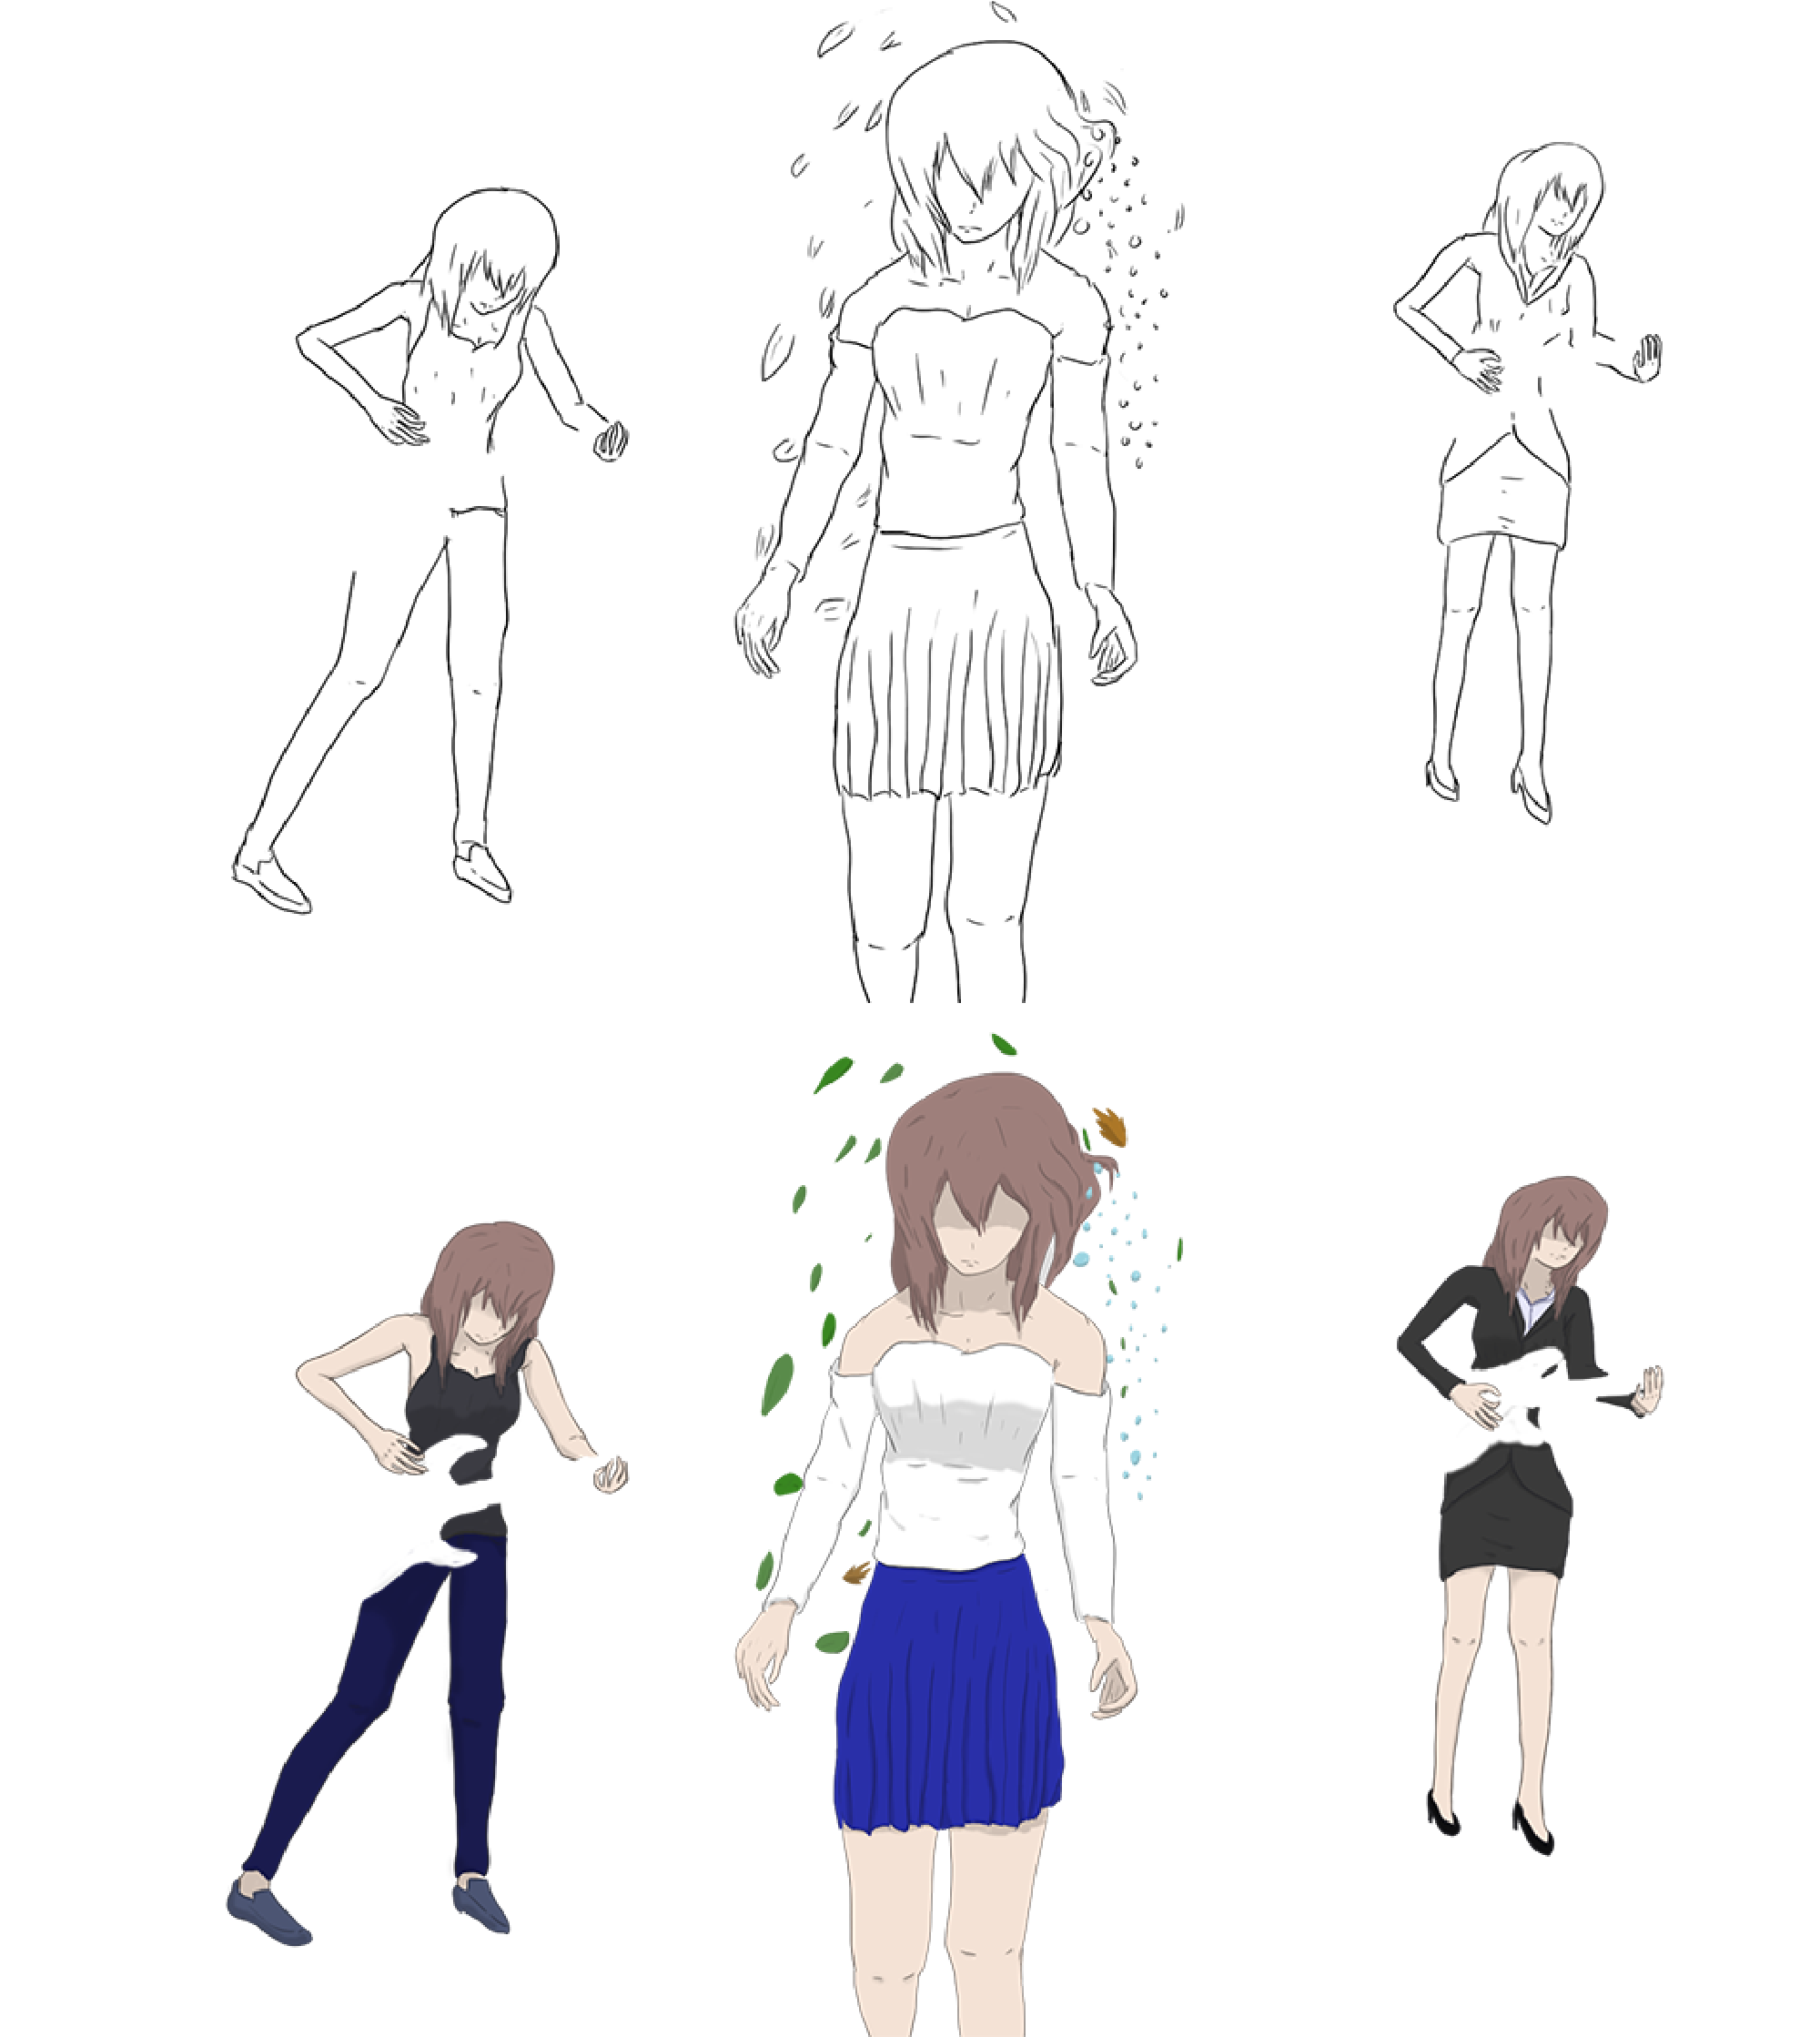
\includegraphics[width=1\linewidth]{img/results/postprocess.pdf} \\
    \caption{\textbf{Top:} {{Hand-drawn lines referencing 3d skeletons and manually-animated particles}} \textbf{Bottom:} {{Post-processed lines with colour, shadows, and particles}}.}
    \vspace{-15pt}
    \label{fig:postprocess}
\end{figure}

Further investigation on how parts of the process of this stage can be automated or improved.\\\\

There are some deep learning libraries that can do both the shadows and colouring, such as style2paints~\cite{style2paintsArxiv} and Preferred Network's PaintsChainer~\cite{paintsChainer} and similar implementations~\cite{autoPainter}. However, since these models were trained for single images, the lack of consistency for usage in animation makes it less viable. Research on additional recurrent neural network layers and retraining for these models are needed before they can be viable for use in animation.

\subsection{Commercial Use and Impact}

As discussed above, only the methods used for creating Brighter the Animation is possible for commercial use, since these do not make use of copyrighted material for training machine learning models nor do they require any expensive licensing. However, after the feasibility of automating parts of the process, use on actual commercial environment can be done, and the effectiveness can be tested and measured to try to solve the problems in the current issues with anime industry. In addition, having the potential of applying machine learning models in the more advanced phases after creating own datasets to avoid copyright infringement introduces more options for automation. The findings in the study can then be applied on a production environment to focus on the three main aspects of anime production targetted by this paper:\\
\begin{enumerate}
    \item Automation of Repetitive, Low-level Tasks
    \begin{itemize}
        \item With the current pipeline, a huge block of the process can already be reduced and the ability to proceed with the Production stage concurrently with sound, music, and dubbing can greatly reduce turnaround time with output
        \item Addition of more advanced motion capture technologies that also include facial expressions will exponentially improve this method, as opposed to the current process where only the bodily movements are captured
    \end{itemize}

    \item Work Environment
    \begin{itemize}
        \item Animators can get a higher wage and the decreased need for additional members since lower-level tasks are now modularised
        \item Since animators do not have dead time where there is no work, a company that applies this pipeline can now hire full-time employees, following most processes by Kyoto Animation as discussed in the previous sections, which makes it conducive for building a career in a more stable manner
        \item In the best case, the animators can even be trained on working with ML or SE on their own, or have the extra time work on improving their art for un-automated tasks such as surreal art creation, non-human animation, backgrounds
        \item On the edge case where there is really nothing to do, animators can simply take courses, create their own scripts for pipeline, research on improving the current processes, or improve their imaginative and artistic abilities
    \end{itemize}

    \item Lessening the Stigma on Anime/Otaku culture
    \begin{itemize}
        \item As discussed previously, with work/life balance, animators can have grounding on real life with their art if they have more life experiences other than simply working day and night on animation.
        \item Some personal notes on this include:
        \begin{itemize}
            \item I believe having a concrete basis that is grounded on real life gives more input features for animators to include when thinking about animation and creating artworks.
            \item Anime and filmmaking as an art is not merely drawing beautiful frames but tackles the complexity of real life issues, human interaction, and the psychology of behavior
            \item With the current stigma on otaku culture, personally I would like to build a community that creates anime movies and series with more basis on real life, international influences including western and Asian culture, and deeper levels of nuance. The themes can vary but the acceptance criteria should always be strict in the sense that it should not just be a recurring-theme anime targetted to exploit primary human needs (e.g. - too much fanservice, unrealistic love stories, cliche). As media and entertainment people that can share information to the world on a larger scale, I think it's also a great opportunity to treat this as conveying different walks of life to both entertain and educate people on both current and historical events \& the human psyche, and motivate learning \& growth
        \end{itemize}
    \end{itemize}
\end{enumerate}